\input{../../../headers/dsheaders.tex}

\subsection*{Présentation}

\subsubsection*{La société : TEAM ASSOCIATED}

\begin{figure}[!ht]
\begin{minipage}[t]{0.65\linewidth}
La société TEAM ASSOCIATED est spécialisée depuis 1965 dans la conception, la fabrication et la vente de modèles réduits radiocommandés (figure \ref{fig01}). Les modèles peuvent prendre différentes formes (avions, voitures, etc.) et différentes échelles (du 1/18 au 1/8).

Les ingénieurs de la société, souvent aussi compétiteurs, apportent leur expertise afin de produire des modèles de plus en plus performants.
\end{minipage}\hfill
\begin{minipage}[t]{0.3\linewidth}
\vspace{-10pt}
\centering
\includegraphics[width=.9\linewidth]{img/fig01}
\caption{\label{fig01}Produits de la société Team Associated}
\end{minipage}
\end{figure}

\vspace{-30pt}

\subsubsection*{Le système étudié : buggy 1/10 radiocommandé}

Le système d'étude choisi est un buggy de compétition à l'échelle 1/10. Sa référence est RC10 B6.3D (figure \ref{fig02}). Il s'agit d'un buggy à deux roues motrices, propulsé par les roues arrière par le biais d'un moteur brushless. Sa longueur est de 460 mm.

Ce buggy est utilisé lors de compétitions nationales et internationales sur des pistes spécifiques (figure \ref{fig03}) où les compétiteurs doivent faire le plus de tours possibles sur une durée de 5 minutes. Cette piste possède différents revêtements (terre, moquette, pavés, etc.) ainsi que plusieurs sauts et bosses.

La maniabilité du buggy et sa tenue de route sont des critères de performance essentiels pour les compétiteurs.

\begin{figure}[!ht]
\begin{minipage}{.5\linewidth}
\vspace{0pt}
\centering
\includegraphics[width=.8\linewidth]{img/fig02}
\caption{\label{fig02}Buggy RC10 B6.3D}
\end{minipage}
\hfill
\begin{minipage}{.5\linewidth}
\vspace{0pt}
\centering
\includegraphics[width=.9\linewidth]{img/fig03}
\caption{\label{fig03}Piste de course de buggy}
\end{minipage}
\end{figure}

L'\textbf{annexe 1 }présente les principaux composants de la voiture.

L'\textbf{annexe 2 }présente plusieurs diagrammes SysML détaillant la constitution et les exigences liées à la voiture.

~\

Le sujet portera sur l'étude de la direction, de la propulsion et de l'équilibre de la voiture lors d'un saut.

\newpage

\section{Exigence 1 : diriger la voiture}

\subsection{Objectif}

Cette partie a pour objectif d'étudier la cinématique de la direction de la voiture afin de valider les exigences 1.2 \og Orienter les roues\fg\ et 1.3 \og Se positionner rapidement\fg\ (figure \ref{fig37}, annexe 2).

\subsection{Étude de la cinématique de direction}

Les paragraphes suivants présentent la chaîne cinématique permettant d'orienter les roues avant du buggy.

Lorsqu'un buggy roule, les roues avant tournent par rapport aux fusées de roue (figure \ref{fig04}) qui guident en rotation leurs axes. Lors d'un virage, chaque fusée pivote par rapport au porte fusée selon l'axe de fusée pour modifier la trajectoire du véhicule. L'orientation du porte fusée dépend de la position de la biellette de direction.

\begin{figure}[!ht]
\centering
\includegraphics[width=.55\linewidth]{img/fig04}
\caption{\label{fig04}Éléments constitutifs de la direction}
\end{figure}

Encastré sur le châssis, un servomoteur (figure \ref{fig05}), équipé d'un palonnier, déplace la biellette de servomoteur. Celle-ci est en liaison sphérique avec un des deux palonniers de direction.

\begin{figure}[!ht]
\centering
\includegraphics[width=.55\linewidth]{img/fig05}
\caption{\label{fig05}Détail des éléments de direction autour du servomoteur}
\end{figure}

Ces palonniers sont en liaison pivot à la fois avec le châssis et avec la barre de direction. La barre de direction est en liaison sphérique avec la biellette de direction.

Pour limiter l'impact des aspérités du sol sur le buggy, ce dernier est équipé de suspensions composées d'amortisseurs à huile et de ressorts visibles sur la figure \ref{fig04}.

Le triangle avant qui supporte le porte fusée est articulé au niveau du châssis. L'amortisseur avant est fixé entre ces deux éléments. Dans le cadre de cette étude, l'amortisseur avant est considéré comme fixe.

Le schéma cinématique simplifié de la direction est donné figure \ref{fig06}. Les liaisons sphériques ont été remplacées par des liaison pivots. Une liaison pivot d'axe (O, $\overrightarrow{z_0}$) entre deux pièces signifie que ces deux pièces ont un mouvement de rotation l'une par rapport à l'autre autour de l'axe (O, $\overrightarrow{z_0}$).

\begin{figure}[!ht]
\centering
\includegraphics[width=\linewidth]{img/fig06}
\caption{\label{fig06}Schéma cinématique de la direction}
\end{figure}

Au châssis $S_0$ est associé le repère $R_0 = (O, \overrightarrow{x_0}, \overrightarrow{y_0}, \overrightarrow{z_0})$. Le châssis est considéré comme fixe.

Les palonniers de direction $S_1$ et $S_2$ sont en liaison pivot d'axe $(O, \overrightarrow{z_0})$ et $(A, \overrightarrow{z_0})$ respectivement avec le châssis. Les repères $R_1 = (O, \overrightarrow{x_1}, \overrightarrow{y_1}, \overrightarrow{z_0})$ et $R_2 = (A, \overrightarrow{x_2}, \overrightarrow{y_2}, \overrightarrow{z_0})$ leurs sont associés. Leurs orientations par rapport à $S_0$ sont définies par les angles orientés $\varphi = (\overrightarrow{y_0}, \overrightarrow{y_1})$ et $\psi = (\overrightarrow{y_0}, \overrightarrow{y_2})$.

À la barre de direction $S_3$ est associé le repère $R_3 = (C, \overrightarrow{x_3}, \overrightarrow{y_3}, \overrightarrow{z_3})$. Cette barre est en liaison pivot d'axe $(C, \overrightarrow{z_0})$ avec $S_1$ et $(D, \overrightarrow{z_0})$ avec $S_2$. Son orientation par rapport au châssis $S_0$ est définie par $\gamma = (\overrightarrow{x_0}, \overrightarrow{x_3})$.

À la biellette de direction $S_4$ est associé le repère $R_4 = (E, \overrightarrow{x_4}, \overrightarrow{y_4}, \overrightarrow{z_0})$. Son orientation par rapport au châssis $S_0$ est définie par l'angle orienté $\delta = (\overrightarrow{x_0}, \overrightarrow{x_4})$, tel que $\overrightarrow{EG} = P \overrightarrow{x_4}$.

À la fusée $S_5$ est associé le repère $R_5 = (H, \overrightarrow{x_5}, \overrightarrow{y_5}, \overrightarrow{z_0})$. Son orientation par rapport au châssis $S_0$ est définie par l'angle orienté $\theta_R = (\overrightarrow{y_0}, \overrightarrow{y_5})$.

Le repère $R_6 = (I, \overrightarrow{x_5}, \overrightarrow{y_6}, \overrightarrow{z_6})$ est associé à la roue $S_6$. L'angle de la roue par rapport à la fusée est défini par l'angle orienté $\mu = (\overrightarrow{y_5}, \overrightarrow{y_6})$.

$F$ est le point d'ancrage de la biellette de servomoteur sur le palonnier de direction $S_1$.

Différents vecteurs sont définis :
\begin{align*}
\overrightarrow{OA} &= K \overrightarrow{x_0} & \overrightarrow{CD} &= K \overrightarrow{x_3}  & \overrightarrow{DE} &= X_3 \overrightarrow{x_3} + Y_3 \overrightarrow{y_3} & \overrightarrow{FO} &= L_b \overrightarrow{y_1}\\
\overrightarrow{CO} &= L \overrightarrow{y_1} & \overrightarrow{DA} &= L \overrightarrow{y_2} &\overrightarrow{EG} &= P \overrightarrow{x_4} & \overrightarrow{GH} &= Q_x \overrightarrow{x_5} + Q_y \overrightarrow{y_5}
\end{align*}

\question{Vu la géométrie du mécanisme, justifier quel est le mouvement possible de la barre de direction $S_3$ par rapport au châssis $S_0$ ? En déduire une relation entre $\varphi$ et $\psi$.}

\question{Justifier que la trajectoire du point E est un cercle de centre A' et donner les coordonnées de $\overrightarrow{AA'}$ dans $R_0$.}

~\

L'amplitude du mouvement du servomoteur (120°) provoque un déplacement maximal du point F dans la direction $+\overrightarrow{x_0}$, tel que $\overrightarrow{OF} \cdot \overrightarrow{x_0} = \Delta_{Fmax} = 8$ mm.

\question{Sachant que la distance $L_b = 16$ mm, déterminer la valeur numérique maximale de l'angle $\varphi$, notée $\varphi_{max}$, lorsque $\overrightarrow{OF} \cdot \overrightarrow{x_0} = \Delta_{Fmax}$.}

~\

L'abaque (figure \ref{fig38} de l'annexe 3) montre l'évolution des courbes sinus et cosinus.

Quels que soient les résultats obtenus précédemment, nous allons maintenant utiliser le modèle cinématique simplifié présenté sur la figure \ref{fig07}.

\begin{figure}[!ht]
\centering
\includegraphics[width=\linewidth]{img/fig07}
\caption{\label{fig07}Schéma cinématique simplifié}
\end{figure}

Le repère $R_0 = (A', \overrightarrow{x_0}, \overrightarrow{y_0}, \overrightarrow{z_0})$ est associé au châssis fixe $S_0$ avec $\overrightarrow{A'H} = M \overrightarrow{x_0} + N \overrightarrow{y_0}$.

$S_2'$ représente un palonnier de direction virtuel. Le repère $R'_2 = (A', \overrightarrow{x_{2'}}, \overrightarrow{y_{2'}}, \overrightarrow{z_0})$ lui est associé. L'angle orienté $\alpha = (\overrightarrow{y_0}, \overrightarrow{y_{2'}})$ et $\overrightarrow{EA'} = L \overrightarrow{y_{2'}}$ sont définis, $L$ étant le même que précédemment. Les autres grandeurs restent inchangées.

L'angle orienté $\theta_4 = (\overrightarrow{x_0}, \overrightarrow{x_4})$ est définit pour la suite.

Ce modèle va nous permettre de déterminer l'angle de braquage maximal du buggy.

\question{Écrire une fermeture géométrique faisant intervenir les solides $S_0$, $S_2'$, $S_4$ et $S_5$.}

\question{Montrer que :
$$P^2 = (M + Q_y \sin \theta_R - Q_x \cos \theta_R - L \sin \alpha)^2 + (N - Q_y \cos \theta_R - Q_x \sin \theta_R + L \cos \alpha)^2.$$}

Les valeurs numériques utiles sont les suivantes : $L = 30$ mm, $M = 100$ mm, $N = 7$ mm, $P = 88$ mm, $Q_x = 12$ mm, $Q_y = 30$ mm.

Pour déterminer l'angle maximum de braquage $\theta_{Rmax}$ pour $\alpha = -30\degree$ (virage à droite), une résolution numérique de la relation de la question \ref{q5} est envisagée.

Le code python suivant a permis de tracer la figure \ref{fig07b}.
\begin{figure}[!ht]
\begin{minipage}{0.5\linewidth}
\begin{minted}[linenos]{python}
from numpy import sin, cos, pi, linspace
import matplotlib.pyplot as plt

def f(thetaR):
    tR=radian(thetaR)
    a = -30*pi/180  # radian
    L,P = 30,88         # mm
    M,N = 100,7         # mm
    Qx,Qy = 12,30       # mm
    a=M+Qy*sin(tR)-Qx*cos(tR)-L*sin(a)
    b=N-Qy*cos(tR)-Qx*sin(tR)+L*cos(a)
    return P**2-a**2-b**2
    		
def radian(deg):
    return deg*pi/180

thetaR=linspace(20,30,100)
plt.plot(thetaR,f(thetaR))
plt.grid(True)
plt.show()
\end{minted}
\end{minipage}
\hfill
\begin{minipage}{0.5\linewidth}
   \def\svgwidth{\textwidth}
 \centering\input{img/fig07b.pdf_tex}
 \caption{\label{fig07b}Tracé issu du programme python}
\end{minipage}
\end{figure}

\question{Déterminer à partir du script python et du tracé de la figure \ref{fig07b} la valeur de $\theta_{Rmax}$.}

~\

Le rayon de braquage interne d'un véhicule dont les roues avant sont directrices est défini de la manière suivante. Soit un cercle dont le centre est situé sur l'axe de rotation des roues arrière du véhicule. Ce cercle est tangent à la roue avant droite du véhicule lorsque celui-ci tourne à droite avec les roues les plus inclinées possible. Le rayon de braquage interne correspond au rayon de ce cercle.

L'empattement, c'est à dire la distance entre les roues avant et arrière du buggy, est $e = 280$ mm.

Le calcul numérique donne $|\theta_{Rmax}| = 42\degree$.

\question{Réaliser un schéma permettant de définir l'angle de braquage interne. Déterminer l'expression littérale et la valeur numérique du rayon de braquage interne $R_i$ du buggy, effectuer pour cela toutes les approximations nécessaires. Est-ce compatible avec l'exigence 1 ?}

~\

Une étude du schéma cinématique de la figure \ref{fig07} a permis de déterminer la relation suivante:

$$\overrightarrow{V_{E\in S'_2/S_0}}\cdot\overrightarrow{x_4}=\overrightarrow{V_{G\in S_5/S_0}}\cdot\overrightarrow{x_4}$$

\question{Quelle propriété a été utilisée afin d'établir cette relation ?}

Les données cinématiques suivantes sont introduites pour la suite :
\begin{align*}
\overrightarrow{\Omega_{5/0}} &= \dot{\theta}_R\cdot \overrightarrow{z_0} & \overrightarrow{\Omega_{4/0}} &= \dot{\theta}_4\cdot \overrightarrow{z_0} & \overrightarrow{\Omega_{2'/0}} &= \dot{\alpha}\cdot \overrightarrow{z_0}
\end{align*}

\question{Montrer qu'à partir de la relation de la question \ref{q8} on peut écrire:
$$L\cdot\dot{\alpha}\cdot\overrightarrow{x'_2}\cdot\overrightarrow{x_4}=\dot{\theta}_R\cdot(-Q_x\cdot\overrightarrow{y_5}+Q_y\cdot\overrightarrow{x_5})\cdot \overrightarrow{x_4}$$}

\question{Puis la relation:
$$L\cdot\dot{\alpha}\cdot cos(\theta_4-\alpha)=\dot{\theta}_R\cdot(Q_x\cdot sin(\theta_R-\theta_4)+Q_y\cdot cos(\theta_R-\theta_4))$$}

En intelligence artificielle, plus précisément en apprentissage automatique, la méthode des k plus proches voisins est une méthode d’apprentissage supervisé. Une étude de ce type a permis de déterminer les deux courbes suivantes.

\begin{figure}[!ht]
 \begin{minipage}{0.48\textwidth}
   \def\svgwidth{1.1\linewidth}
   \centering\input{img/figthetar.pdf_tex}
   \caption{\label{fig07c}$\theta_R$ ($rad$) et $\theta_4$ (rad) en fonction de $\alpha$ ($rad$)}
 \end{minipage}\hfill
 \begin{minipage}{0.48\textwidth}
   \def\svgwidth{1.1\linewidth}
   \centering\input{img/figomegar.pdf_tex}
   \caption{\label{fig07d}$\dot{\theta}_R$ ($rad\cdot s^{-1}$) en fonction de $\alpha$ ($rad$)}
 \end{minipage}
\end{figure}

\question{Vérifier pour la seule configuration $\theta_4=\theta_R$ que la relation de la question \ref{q10} est vraie.}

\subsection{Étude de l'asservissement du servomoteur}

L'actionneur associé à la direction du buggy est un servomoteur (figure \ref{fig05}). Lorsque le pilote envoie une consigne de position angulaire par le biais de sa télécommande, le palonnier du servomoteur tourne d'un angle proportionnel à la consigne. Les constituants internes de l'actionneur sont visibles sur les figures \ref{fig08} et \ref{fig09}.

\begin{figure}[!ht]
\begin{minipage}{.5\linewidth}
\vspace{0pt}
\centering
\includegraphics[width=.8\linewidth]{img/fig08}
\caption{\label{fig08}Réducteur du servomoteur}
\end{minipage}
\hfill
\begin{minipage}{.5\linewidth}
\vspace{0pt}
\centering
\includegraphics[width=.9\linewidth]{img/fig09}
\caption{\label{fig09}Constituants dans le boîtier du servomoteur}
\end{minipage}
\end{figure}

Lorsque le pilote envoie une consigne de position angulaire $\theta_{Rc}$ par le biais de sa télécommande, le récepteur génère un signal PWM (Pulse Width Modulation) dont le rapport cyclique est proportionnel à l'angle désiré, la compréhension de cet aspect n'est pas nécessaire pour effectuer la suite de l'épreuve. Le gain associé au récepteur est noté $K_{rec}$.

Ce signal électrique est reçu par la carte de contrôle du servomoteur qui est composée :
\begin{itemize}
\item d'un convertisseur de gain $C_o$ qui convertit le signal PWM en tension analogique proportionnelle à l'angle demandé ;
\item d'un comparateur qui compare la tension de commande à la tension de sortie du potentiomètre ;
\item d'un correcteur de gain $K_{cor}$ ;
\item d'un variateur de gain $V_{sm}$.
\end{itemize}

La carte de contrôle alimente, avec une tension $U_s$, le moteur à courant continu. Celui-ci tourne alors à une vitesse de rotation $\omega_{mot}$.

Une fonction de transfert $H_m(p) = \frac{K_m}{1 + \tau_m p}$ est associée au moteur, avec $K_m$ le gain statique du moteur et $\tau_m$ sa constante de temps.

Le rapport de transmission du réducteur est noté $i_{sm} = \frac{\omega_{mot}}{\omega_{red}}$, avec $\omega_{red}$ la vitesse de rotation en sortie du réducteur et $\omega_{mot}$ la vitesse de rotation en sortie du moteur.

Un potentiomètre est placé en sortie du réducteur, c'est-à-dire, sur l'axe du palonnier du servomoteur (figure \ref{fig05}). Il mesure la position angulaire du palonnier $\theta_p$ et renvoie une tension analogique $U_p$ à la carte de contrôle. Un gain $K_p$ lui est associé.

\question{Compléter le schéma bloc de cet asservissement en position angulaire.}

~\

Afin d'identifier le comportement du servomoteur, des essais avec des entrées en échelon ont été effectués. En partant de la position neutre de 0°, une consigne de position angulaire $\theta_{Rc}$ de 30° a été envoyée au servomoteur. La tension de sortie $U_p$ du potentiomètre a été mesurée à l'aide d'un oscilloscope. Après étalonnage, l'évolution de $\theta_p$ a pu être tracée.

L'angle mesuré étant très bruité, il a été filtré à l'aide d'un fonction du premier ordre $H_f(p)$ de fréquence de coupure $f_c = 5$ Hz et de gain 1. La figure \ref{fig10} présente deux courbes. La première est l'évolution temporelle de l'angle mesuré après filtrage. La seconde est l'évolution temporelle de la vitesse angulaire du palonnier.

\question{Tracer le tracé asymptotique du diagramme de Bode de la fonction $H_f(p)$}

\question{De combien de décibels (dB) est atténué un bruit de fréquence de 20 Hz ?}

\begin{figure}[!ht]
\centering
\includegraphics[width=.9\linewidth]{img/fig10}
\caption{\label{fig10}Évolution de l'angle et de la vitesse angulaire du palonnier pour une variation de consigne en échelon de 30°}
\end{figure}

\question{Quel peut être l'ordre de la fonction de transfert dont la réponse à un échelon de 30° est tracée sur la figure \ref{fig10} ? Déterminer le temps de réponse à 5 \%, noté $T_{r5\%}$. Conclure vis-à-vis du cahier des charges.}

La fonction choisie pour identifier ce tracé est :
$$\dfrac{K}{(1+0.05\cdot p)(1+0.08\cdot p)}$$

\question{Justifier que cette fonction est compatible avec le tracé et calculer les valeurs numériques de son gain $K$, de sa pulsation propre $\omega_0$ et de son coefficient d'amortissement $\xi$.}

Afin d'améliorer les performances du système, un correcteur proportionnel de gain $K_{cor}$ est implémenté dans la carte de contrôle en aval du comparateur.

Le schéma bloc de l'asservissement angulaire du potentiomètre est simplifié pour ne présenter qu'un seul bloc issu des mesures précédentes. Ce schéma bloc est représenté sur la figure 11.

\begin{figure}[!ht]
\centering
\includegraphics[width=.7\linewidth]{img/fig11}
\caption{\label{fig11}Schéma bloc simplifié avec correcteur proportionnel}
\end{figure}

Pour la fonction de transfert du système en Boucle Ouverte (BO), les valeurs suivantes sont fixées : $K_{BO} = 6$, $m_{BO} = 3$ et $\omega_{BO} = 5$ rad·s$^{-1}$.

\question{Déterminer l'expression de la fonction de transfert corrigée en boucle fermée $H_c(p) = \frac{\theta_p(p)}{\theta_{Rc}(p)}$ sous forme canonique.}

\question{Donner l'ordre de $H_c(p)$ ainsi que l'expression de son gain statique, noté $G_c$.}

\question{Déterminer l'expression de $K_{cor}$ pour obtenir le système le plus rapide possible sans dépassement. Faire l'application numérique.}

~\

Le correcteur permet d'obtenir un temps de réponse de $T_{r5\%} = 0,1$ s pour 30°.

\question{En faisant l'hypothèse que le système ne sature pas, déterminer le temps de réponse à 5 \%, noté $T_{r60}$ pour un débattement de 60°. Conclure vis-à-vis des exigences du cahier des charges.}

\question{Déterminer l'erreur statique du système corrigée en boucle fermée pour une entrée unitaire.}

~\

Une correction intégrale est ajoutée au correcteur dans la suite, ainsi $K_{cor}=K_p+\dfrac{K_i}{p}$.

\question{Déterminer l'erreur statique du système corrigée en boucle fermée pour une entrée unitaire avec cette nouvelle correction.}

\section{Exigence 3 : mettre en mouvement la voiture}

\subsection{Objectif}

L'objectif de cette partie est d'analyser le différentiel à bille qui fait partie du train arrière permettant de propulser la voiture.

\subsection{Étude du différentiel à billes}

Le différentiel à billes est composé de quatorze billes réparties dans une couronne centrale. Deux plateaux viennent en contact de chaque côté et sont plaqués par un ressort.

\begin{figure}[!ht]
\begin{minipage}{.5\linewidth}
\vspace{0pt}
\centering
\includegraphics[width=.8\linewidth]{img/fig25}
\caption{\label{fig25}Différentiel monté dans la voiture}
\end{minipage}
\hfill
\begin{minipage}{.5\linewidth}
\vspace{0pt}
\centering
\includegraphics[width=.9\linewidth]{img/fig26}
\caption{\label{fig26}Éclaté du différentiel}
\end{minipage}
\end{figure}

Afin de simplifier l'étude, le réglage de précontrainte réalisé par le ressort et l'écrou est fixé. Un schéma cinématique simplifié est donné sur la figure \ref{fig27}.

\begin{figure}[!ht]
\centering
\includegraphics[width=.8\linewidth]{img/fig27}
\caption{\label{fig27}Schéma cinématique simplifié du différentiel}
\end{figure}

Hypothèses et données :
\begin{itemize}
\item une seule bille $S_4$ est utilisée pour la modélisation ;
\item $\overrightarrow{V_{C\in 4/3}}=\overrightarrow{0}$,
\item il y a roulement sans glissement en I et J entre la bille $S_4$ et les plateaux $S_1$ et $S_2$ ;
\item à chaque solide $S_i$ est lié un repère $R_i = (O, \overrightarrow{x}_i, \overrightarrow{y}_i, \overrightarrow{z}_0)$ ;
\item $\overrightarrow{OC} = R \overrightarrow{x}_3$ ;
\item $\overrightarrow{CJ} = -r \overrightarrow{z}_0$ et $\overrightarrow{CI} = r \overrightarrow{z}_0$ ;
\item $\omega_{i0}$ est définie pour tout i par $\omega_{i0} = \dot{\theta}_{i0}$.
\end{itemize}

\question{Réaliser le graphe des liaisons du mécanisme.}

\question{Établir une relation entre $\overrightarrow{V}_{J,4/3}$ et $\overrightarrow{V}_{I,4/3}$ en écrivant une égalité de vitesses au point C.}

~\

La vitesse de rotation du solide $S_i$ par rapport au solide $S_j$ est notée $\omega_{ij}$.

\question{Écrire la relation de roulement sans glissement en I et en déduire une expression de $\overrightarrow{V}_{I,4/3}$ en fonction de $\omega_{31}$ et de R.}

\question{Écrire la relation de roulement sans glissement en J et en déduire une expression de $\overrightarrow{V}_{J,4/3}$ en fonction de $\omega_{32}$ et de R.}

\question{Dans le cas où la couronne centrale $S_3$ est bloquée, c'est-à-dire avec $\omega_{30} = 0$, déterminer la relation entre les vitesses de rotation $\omega_{10}$ du plateau gauche $S_1$ et $\omega_{20}$ du plateau droit $S_2$ par rapport au bâti $S_0$.}

\question{En faisant l'hypothèse que la roue droite tourne deux fois moins vite que la roue gauche, $\omega_{10} = 2 \cdot \omega_{20}$, déterminer la relation entre les vitesses de rotation $\omega_{10}$ du plateau gauche $S_1$ et $\omega_{30}$ de la couronne centrale $S_3$ par rapport au bâti $S_0$.}

\question{Quel est l'intérêt d'utiliser un différentiel sur les roues motrices d'une voiture ? Quelle est l'exigence satisfaite par ce composant ?}

\clearpage

\section*{ANNEXE 1 - Principaux composants de la voiture}

\begin{figure}[!ht]
\centering
\includegraphics[width=.8\linewidth]{img/fig33}
\caption{\label{fig33}Buggy RC10 B6.3D avec annotations}
\end{figure}

\clearpage

\section*{ANNEXE 2 - Diagrammes SysML}

\begin{figure}[!ht]
\begin{minipage}[t]{0.5\linewidth}
\vspace{0pt}
\centering
\includegraphics[width=.8\linewidth]{img/fig34}
\caption{\label{fig34}Diagramme des cas d'utilisation}
\end{minipage}\hfill
\begin{minipage}[t]{0.5\linewidth}
\vspace{0pt}
\centering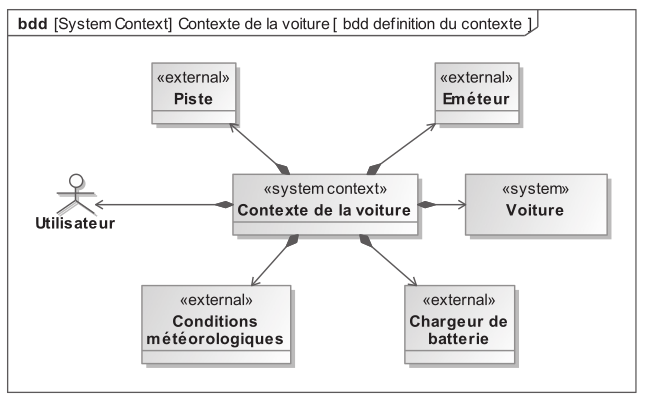
\includegraphics[width=.8\linewidth]{img/fig35}
\caption{\label{fig35}Diagramme de contexte}
\end{minipage}
\end{figure}

\begin{figure}[!ht]
\centering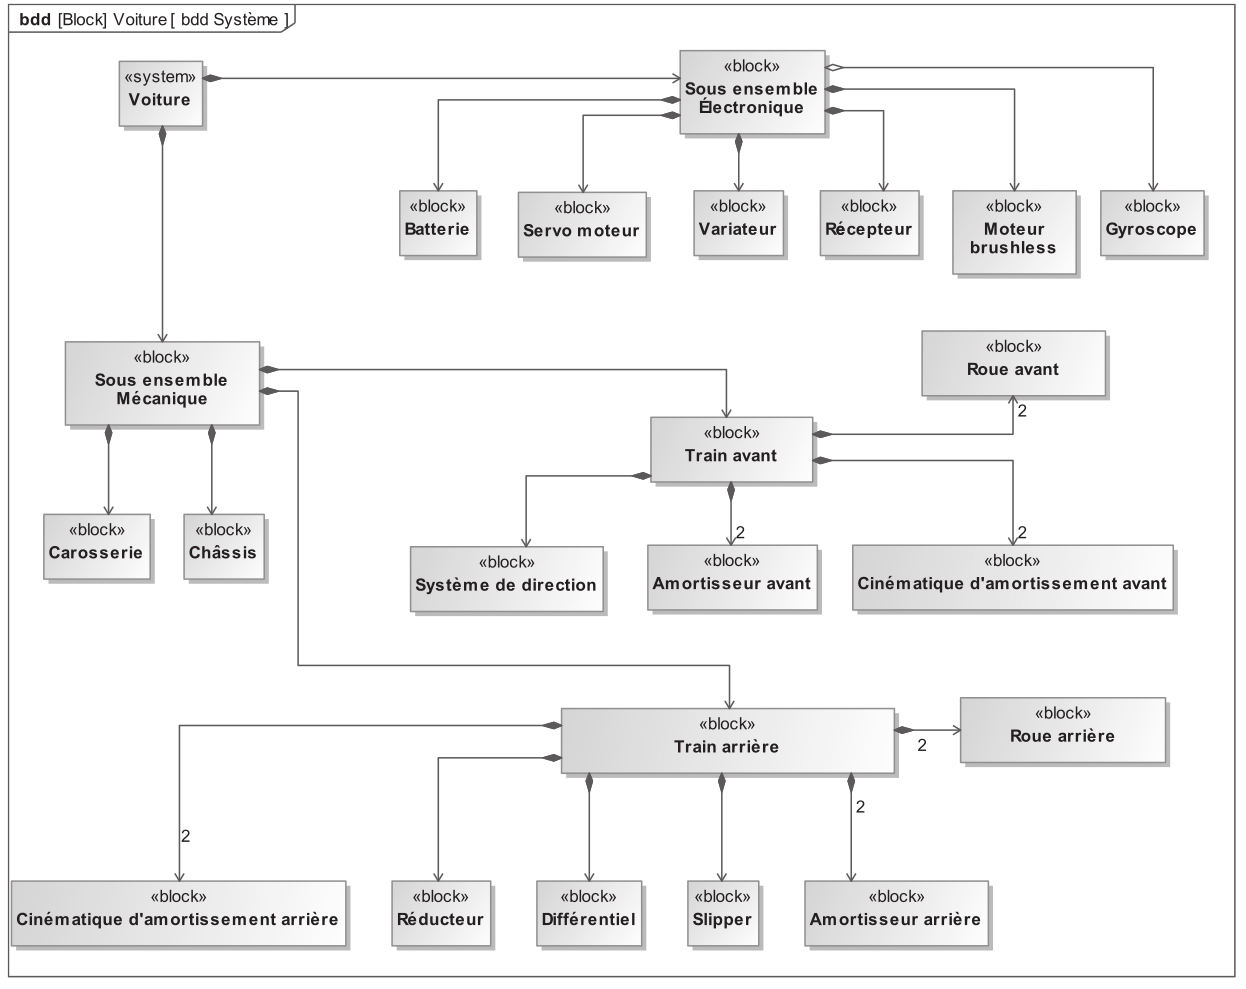
\includegraphics[width=.8\linewidth]{img/fig36}
\caption{\label{fig36}Diagramme de définition de bloc}
\end{figure}

\begin{figure}[!ht]
\centering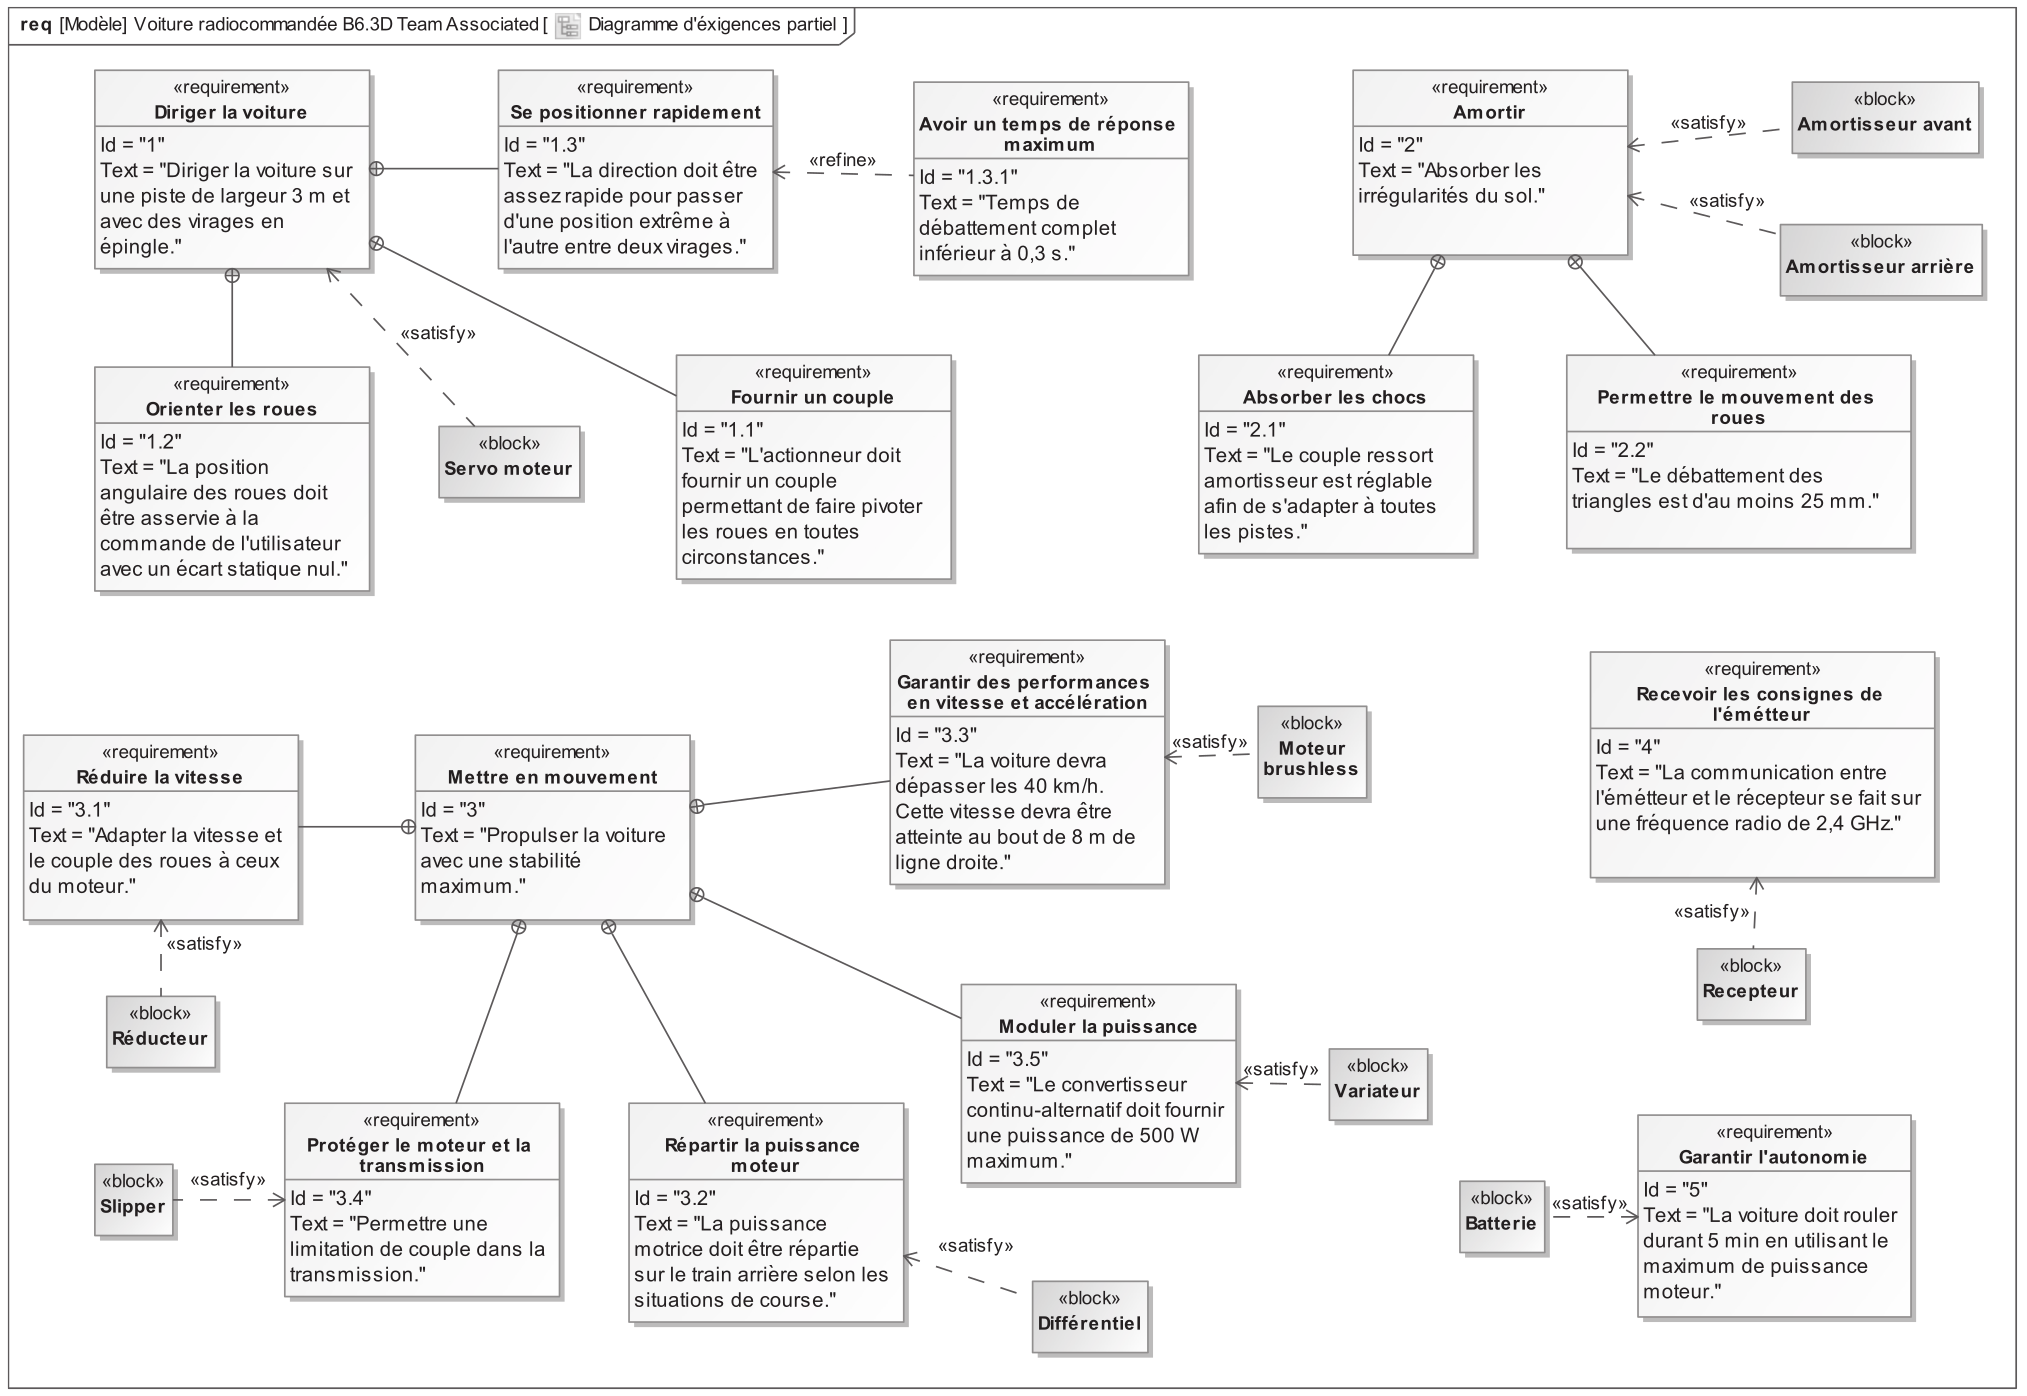
\includegraphics[width=1.3\linewidth,angle=90]{img/fig37}
\caption{\label{fig37}Diagramme partiel des exigences}
\end{figure}

\clearpage

\section*{ANNEXE 3 - Abaque des fonctions sinus et cosinus}

\begin{figure}[!ht]
\centering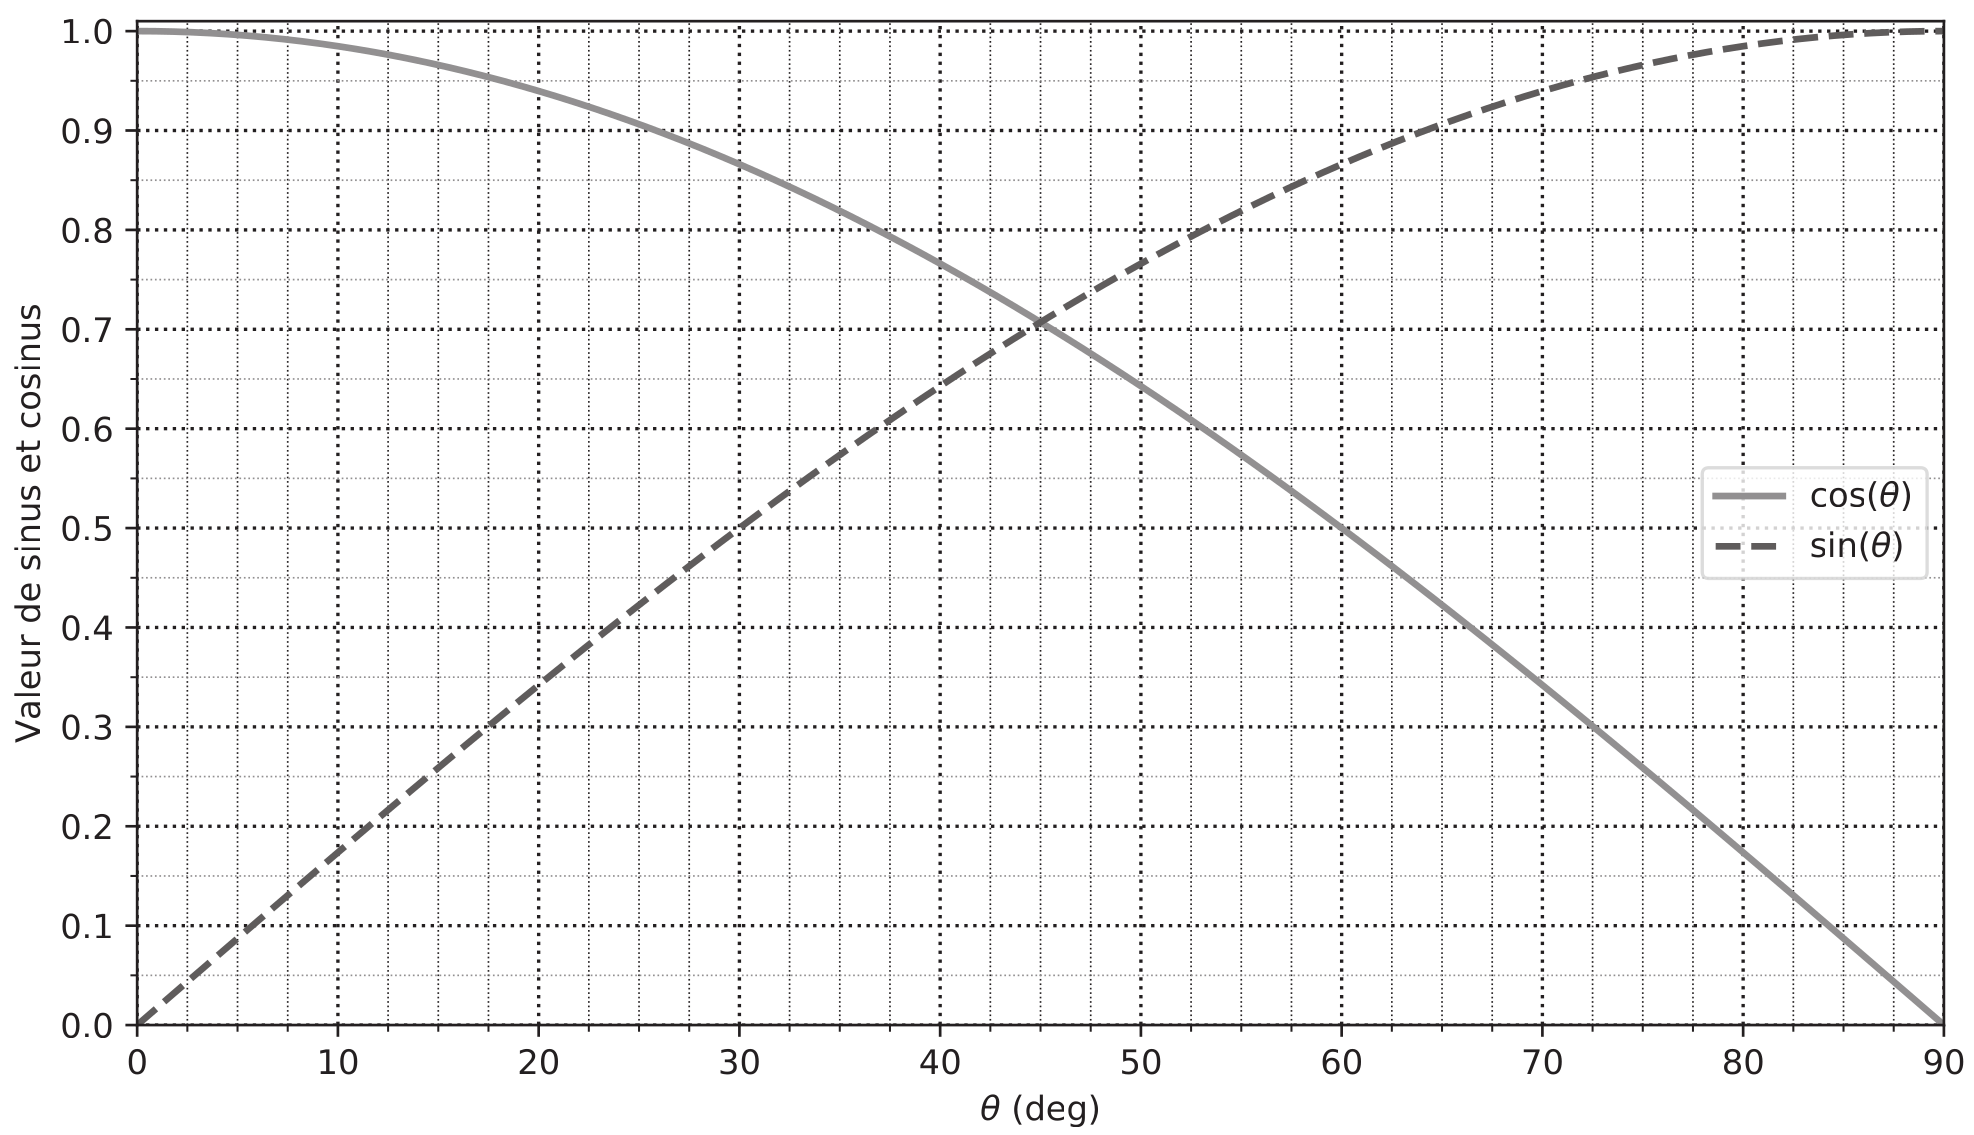
\includegraphics[width=.8\linewidth]{img/fig38}
\caption{\label{fig38}Graphique sin/cos de 0 à 90 degrés}
\end{figure}

\finsujet

\sautpage{1}
\debutcor

\reponse{4}{}{Le quadrilatère $OADC$ a ses côtés opposés de même longueur ($OA = CD = K$ et $OC = AD = L$) : c'est donc un parallélogramme, et ses côtés opposés sont toujours parallèles. On a donc :
\begin{itemize}
\item $\overrightarrow{x_3} = \overrightarrow{x_0}$ : la barre de direction $S_3$ a un mouvement de translation circulaire de rayon $L$ par rapport au châssis $S_0$ ;
\item $\overrightarrow{y_1} = \overrightarrow{y_2}$, et donc $\varphi = \psi$.
\end{itemize}}

\reponse{4}{}{D'après la question précédente, la trajectoire du point $E$ (appartenant à $S_3$ dans son mouvement par rapport à $S_0$) est donc un cercle, de rayon $L$ et de centre $A'$ tel que $\vect{AA'} = \overrightarrow{DE} = X_3\overrightarrow{x_0}+Y_3\overrightarrow{y_0}$.}

\reponse{4}{}{\[
\sin(\varphi) = \frac{\overrightarrow{OF} \cdot \overrightarrow{x_0}}{\|\overrightarrow{OF}\|} = \frac{\Delta_{Fmax}}{L_b} = \frac{1}{2} \Rightarrow \varphi_{max} = 30°
\]}

\reponse{4}{}{\[
\overrightarrow{0} = \overrightarrow{A'H} + \overrightarrow{HG} + \overrightarrow{GE} + \overrightarrow{EA'} = M\overrightarrow{x_0} + N\overrightarrow{y_0} - Q_x\overrightarrow{x_5} - Q_y\overrightarrow{y_5} - P\overrightarrow{x_4} + L\overrightarrow{y_2'}
\]}

\reponse{6}{}{En projetant l'équation obtenue à la question précédente sur les vecteurs du repère $\mathcal{R}_0$ :

\begin{align*}
\text{Sur } \overrightarrow{x_0} : \quad & 0 = M - Q_x \cos(\theta_R) + Q_y \sin(\theta_R) - P \cos(\delta) - L \sin(\alpha)\\
\text{Sur } \overrightarrow{y_0} : \quad & 0 = N - Q_x \sin(\theta_R) - Q_y \cos(\theta_R) - P \sin(\delta) + L \cos(\alpha)
\end{align*}

D'où :
\[
\begin{cases}
P \cos(\delta) = M - Q_x \cos(\theta_R) + Q_y \sin(\theta_R) - L \sin(\alpha)\\
P \sin(\delta) = N - Q_x \sin(\theta_R) - Q_y \cos(\theta_R) + L \cos(\alpha)
\end{cases}
\]

En élevant au carré chacune de ces équations, puis en les sommant, puisque $\cos(\delta)^2 + \sin(\delta)^2 = 1$, on obtient alors bien l'expression demandée.}

\reponse{2}{}{Par lecture l'ordonnée vaut 0 pour $\theta_{Rmax}=42\degree$}

\reponse{8}{}{On supposera que la voie avant (c'est-à-dire la distance entre les deux roues avants) et la voie arrière sont les mêmes, ce qui semble probable d'après la photographie en annexe 1.

   \def\svgwidth{.7\linewidth}
   \centering\input{img/cor07.pdf_tex}

On constate que l'angle de braquage interne est égal à l'angle maximum de braquage (angles alternes-internes), et on a dès lors, en constatant que $\sin(\theta_{Rmax}) = \sin(42\degree) \approx \frac{2}{3}$ :

\[
R_i = \frac{e}{\sin(\theta_{Rmax})} = 420 \text{ mm}
\]

Cela est bien compatible avec l'exigence 1, qui impose de pouvoir diriger la voiture sur des pistes de 3 m de large avec des virages en épingle. Dans un tel virage, le rayon de courbure est maximal à l'extérieur du virage et vaut 3 m, auquel il faut soustraire la largeur du buggy, mais dont le résultat reste largement supérieur à $R_i$.}

\reponse{4}{}{Il s'agit de l'application du principe de l'équiprojectivité au mouvement de 4/0 aux points E et G. Ensuite, on sait que $\overrightarrow{V_{E\in S_4/S_{2'}}}=\overrightarrow{0}$ et $\overrightarrow{V_{E\in S_4/S_5}}=\overrightarrow{0}$, on retrouve alors la formule demandée.}

\reponse{5}{}{Soit $\overrightarrow{V_{E\in S_{2'}/S_0}}.\overrightarrow{x_4}=\overrightarrow{V_{G\in S_5/S_0}}.\overrightarrow{x_4}$,
 
$\overrightarrow{V_{E\in S_{2'}/S_0}}=\overrightarrow{V_{A'\in S_{2'}/S_0}}+\overrightarrow{EA'}\wedge \overrightarrow{\Omega_{2'/0}}=L\cdot\overrightarrow{y'_2}\wedge \dot{\alpha}\overrightarrow{z_0}=L\cdot \dot{\alpha} \cdot \overrightarrow{x'_2}$

$\overrightarrow{V_{G\in S_5/S_0}}=\overrightarrow{V_{H\in S_5/S_0}}+\overrightarrow{GH}\wedge \overrightarrow{\Omega_{5/0}}=(Q_x\overrightarrow{x_5}+Q_y\overrightarrow{y_5})\wedge \dot{\theta}_R\overrightarrow{z_0}=\dot{\theta}_R\cdot (-Q_x\overrightarrow{y_5}+Q_y\overrightarrow{x_5})$

$L\cdot \dot{\alpha} \cdot \overrightarrow{x'_2}.\overrightarrow{x_4}=\dot{\theta}_R\cdot (-Q_x\overrightarrow{y_5}+Q_y\overrightarrow{x_5})\cdot\overrightarrow{x_4}$
}


\reponse{5}{}{$\overrightarrow{x'_2}\cdot\overrightarrow{x_4}=cos(\theta_4-alpha)$

$\overrightarrow{y_5}\cdot\overrightarrow{x_4}=sin(\theta_R-\theta_4)$

$\overrightarrow{x_5})\cdot\overrightarrow{x_4}=cos(\theta_R-\theta_4)$

$L\cdot \dot{\alpha} \cdot cos(\theta_4-\alpha)=\dot{\theta}_R\cdot (Q_x\cdot sin(\theta_R-\theta_4)+Q_y\cdot cos(\theta_R-\theta_4))$
}

\reponse{5}{}{Si $\theta_R=\theta_4$, alors $\alpha=0.1rad$ et $\theta_R=\theta_4=0.1rad$ d'après la figure \ref{fig07c}.

De plus, $L\cdot \dot{\alpha} \cdot cos(\theta_4-\alpha)=\dot{\theta}_R\cdot (Q_x\cdot sin(\theta_R-\theta_4)+Q_y\cdot cos(\theta_R-\theta_4))$ devient $L\cdot \dot{\alpha} = \dot{\theta}_R\cdot Q_y$

Soit $\dot{\theta}_R=\dfrac{L\cdot \dot{\alpha}}{Q_y}$ or $L=Q_y=30mm$, donc $\dot{\theta}_R=\dot{\alpha}=0.07rad\cdot s^{-1}$, on retrouve bien la valeur sur la courbe \ref{fig07d}.
}

\reponse{0}{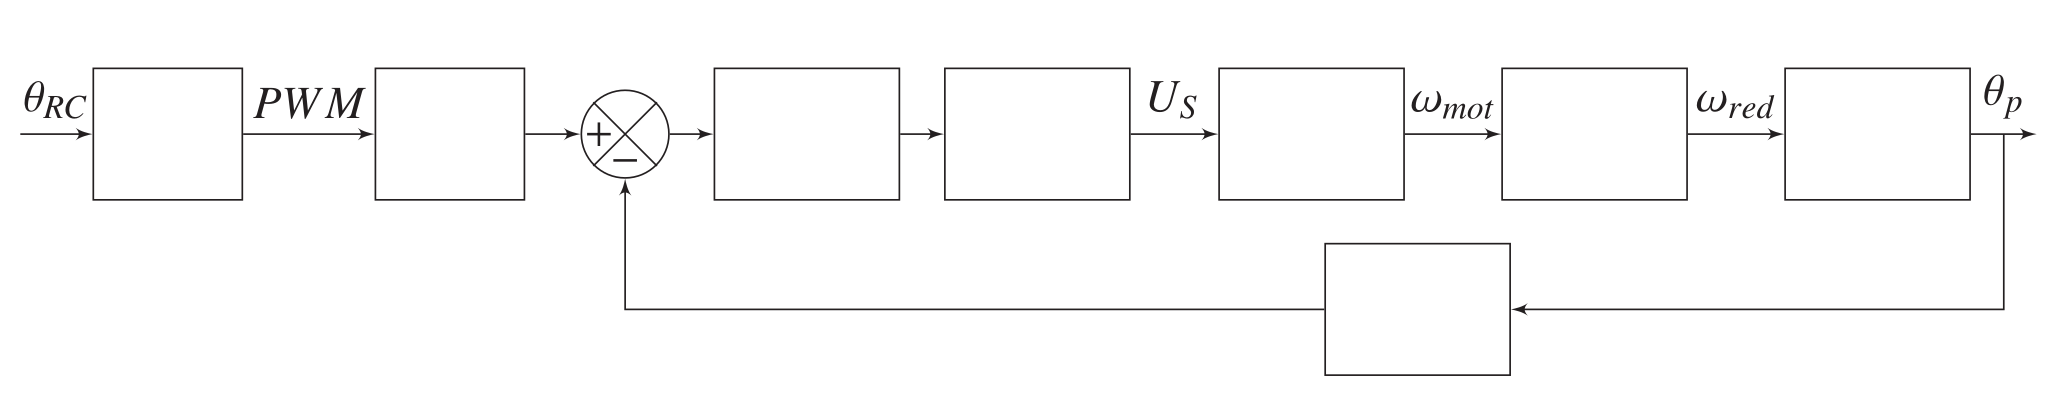
\includegraphics[width=\linewidth]{img/dr12}}{~\ 
	
   \def\svgwidth{\linewidth}
   \centering\input{img/cor12.pdf_tex}
}


\reponse{0}{~\ 
	
   \def\svgwidth{\linewidth}
   \centering\input{img/dr13.pdf_tex}
}{~\ 
	
   \def\svgwidth{\linewidth}
   \centering\input{img/cor13.pdf_tex}
}

\reponse{4}{}{On lit graphiquement sur le tracé précédent, à une fréquence de 20 Hz, soit $\approx 120rad\cdot s^{-1}$, un gain $G_{dB} = -12$ dB.}

\reponse{4}{}{On constate, sur la première courbe de la figure 10, que la réponse du système à un échelon possède une tangente horizontale à l'origine. La fonction de transfert associée est donc au moins d'ordre 2.

La réponse tend vers 26°. On détermine donc graphiquement le temps de réponse à 5\%, c'est-à-dire le temps pour que la réponse entre dans l'intervalle $[24,7 ; 27,3]$ sans en ressortir : $T_{r5\%} = 0,2$ s $< 0,3$ s. Donc, l'exigence 1.3.1 est donc respectée.}

\reponse{2}{}{$K=\dfrac{28}{30}\approx 0.9$

$\omega_0=\dfrac{1}{0.05\cdot 0.08}=20*12.5=250rad\cdot s^{-1}$

$\xi=\dfrac{\omega_0}{2}\cdot 0.13=125*0.13=13+3.25=16.25$}

\reponse{7}{}{
\[
FTBO_c(p) = \frac{K_{cor}K_{BO}}{1 + \frac{2m_{BO}}{\omega_{BO}}p + \frac{1}{\omega_{BO}^2}p^2}
\]

Donc :
\[
H_c(p) = \frac{FTBO_c(p)}{1 + FTBO_c(p)} = \frac{K_{cor}K_{BO}}{K_{cor}K_{BO} + 1 + \frac{2m_{BO}}{\omega_{BO}}p + \frac{1}{\omega_{BO}^2}p^2}
\]

\[
= \frac{\frac{K_{cor}K_{BO}}{1 + K_{cor}K_{BO}}}{1 + \frac{2m_{BO}}{\omega_{BO}(1 + K_{cor}K_{BO})}p + \frac{1}{\omega_{BO}^2(1 + K_{cor}K_{BO})}p^2}
\]}

\reponse{2}{}{$H_C(p)$ est donc une fonction \textbf{d'ordre 2} et $G_c = \frac{K_{cor}K_{BO}}{1+K_{cor}K_{BO}}$.}

\reponse{8}{}{Pour un système d'ordre 2, la réponse la plus rapide possible sans dépassement est obtenue pour un facteur d'amortissement égal à 1. Or :

\begin{align*}
\frac{1}{\omega_{BF}^2} &= \frac{1}{\omega_{BO}^2(1 + K_{cor}K_{BO})} \Leftrightarrow \omega_{BF} = \omega_{BO}\sqrt{1 + K_{cor}K_{BO}}\\
\frac{2m_{BF}}{\omega_{BF}} &= \frac{2m_{BO}}{\omega_{BO}(1 + K_{cor}K_{BO})} \Leftrightarrow m_{BF} = \frac{\omega_{BF}}{\omega_{BO}} \cdot \frac{m_{BO}}{1 + K_{cor}K_{BO}} = \frac{m_{BO}}{\sqrt{1 + K_{cor}K_{BO}}}
\end{align*}

Donc :
\[
m_{BF} = \frac{m_{BO}}{\sqrt{1 + K_{cor}K_{BO}}} = 1 \Rightarrow 1 + K_{cor}K_{BO} = m_{BO}^2
\]
\[
\Leftrightarrow K_{cor} = \frac{m_{BO}^2 - 1}{K_{BO}} = \frac{9 - 1}{6} = 1,33
\]}

\reponse{3}{}{Puisqu'on ne prend pas en compte de saturation, le système est linéaire, continu et invariant donc le temps de réponse ne dépend alors pas de l'amplitude de la consigne : $T_{r60} = T_{r5\%} = 0,1$ s $< 0,3$ s donc, l'exigence 1.3.1 est respectée.}

\reponse{4}{}{
$
\lim\limits_{t\to +\infty} \epsilon(t)=\lim\limits_{p\to 0} p\cdot \epsilon(p)=\lim\limits_{p\to 0} p\cdot (\theta_{Rc}(p)-\theta_R(p))=\lim\limits_{p\to 0} p\cdot (\dfrac{1}{p}-H_c(p)\cdot \dfrac{1}{p})
=\lim\limits_{p\to 0} 1-H_c(p)=1-\frac{K_{cor}K_{BO}}{1 + K_{cor}K_{BO}}
=\frac{1}{1 + K_{cor}K_{BO}}\neq 0$ donc le cahier des charges n'est pas validé.
}

\reponse{5}{}{
Si $K_{cor}=K_p+\frac{K_i}{p}$ alors 

$H_c(p)= \frac{\left(K_p+\frac{K_i}{p}\right)\cdot K_{BO}}{\left(K_p+\frac{K_i}{p}\right)\cdot K_{BO} + 1 + \frac{2m_{BO}}{\omega_{BO}}p + \frac{1}{\omega_{BO}^2}p^2}$

$H_c(p)= \frac{\left(K_p\cdot p+K_i\right)\cdot K_{BO}}{\left(K_p\cdot p+K_i\right)\cdot K_{BO} + p + \frac{2m_{BO}}{\omega_{BO}}p^2 + \frac{1}{\omega_{BO}^2}p^3}$

$
\lim\limits_{t\to +\infty} \epsilon(t)=\lim\limits_{p\to 0} 1-H_c(p)=1-\frac{K_i\cdot K_{BO}}{K_i\cdot K_{BO}}=0$, dans ce cas, le cahier des charges est validé.}

\reponse{5}{}{
Attention bien que suffisant pour ce DS car nous ne l'avons pas encore vu en classe, ce graphe des liaisons ne sera plus suffisant dans les prochaines semaines.
	
   \def\svgwidth{.5\linewidth}
   \centering\input{img/cor23.pdf_tex}
}

\reponse{6}{}{Le point $C$ étant le centre de la liaison rotule entre la couronne $S_3$ et la bille $S_4$, on a :
\[
\overrightarrow{V}_{C,4/3} = \overrightarrow{0}
\]

Or, d'une part :
\[
\overrightarrow{V}_{I,4/3} = \overrightarrow{V}_{C,4/3} + \overrightarrow{IC} \wedge \overrightarrow{\Omega}_{4/3} = \overrightarrow{IC} \wedge \overrightarrow{\Omega}_{4/3}
\]

Et, d'autre part, puisque $\overrightarrow{JC} = -\overrightarrow{IC}$ :
\[
\overrightarrow{V}_{J,4/3} = \overrightarrow{V}_{C,4/3} + \overrightarrow{JC} \wedge \overrightarrow{\Omega}_{4/3} = -\overrightarrow{IC} \wedge \overrightarrow{\Omega}_{4/3}
\]

D'où :
\[
\overrightarrow{V}_{I,4/3} = -\overrightarrow{V}_{J,4/3}
\]
}

\reponse{6}{}{La bille $S_4$ roulant sans glisser sur le plateau $S_1$, on a :
\[
\overrightarrow{V}_{I,4/1} = \overrightarrow{0}
\]

Or, $\overrightarrow{V}_{I,4/1} = \overrightarrow{V}_{I,4/3} + \overrightarrow{V}_{I,3/1}$ et :
\begin{align*}
\overrightarrow{V}_{I,3/1} &= \overrightarrow{V}_{O,3/1} + \overrightarrow{IO} \wedge \overrightarrow{\Omega}_{3/1}\\
&= \overrightarrow{0} + (-r\overrightarrow{z_0} - R\overrightarrow{x_3}) \wedge (\omega_{31}\overrightarrow{z_0})\\
&= R\omega_{31}\overrightarrow{y_3}
\end{align*}

Donc :
\[
\overrightarrow{V}_{I,4/3} = -R\omega_{31}\overrightarrow{y_3}
\]}

\reponse{6}{}{La bille $S_4$ roulant sans glisser sur le plateau $S_2$, on a :
\[
\overrightarrow{V}_{J,4/2} = \overrightarrow{0}
\]

Or, $\overrightarrow{V}_{J,4/2} = \overrightarrow{V}_{J,4/3} + \overrightarrow{V}_{J,3/2}$, et :
\begin{align*}
\overrightarrow{V}_{J,3/2} &= \overrightarrow{V}_{O,3/2} + \overrightarrow{JO} \wedge \overrightarrow{\Omega}_{3/2}\\
&= \overrightarrow{0} + (r\overrightarrow{z_0} - R\overrightarrow{x_3}) \wedge (\omega_{32}\overrightarrow{z_0})\\
&= R\omega_{32}\overrightarrow{y_3}
\end{align*}

Donc :
\[
\overrightarrow{V}_{J,4/3} = -R\omega_{32}\overrightarrow{y_3}
\]}

\reponse{6}{}{Dans le cas où la couronne centrale $S_3$ est bloquée, c'est-à-dire avec $\omega_{30} = 0$, déterminer la relation entre les vitesses de rotation $\omega_{10}$ du plateau gauche $S_1$ et $\omega_{20}$ du plateau droit $S_2$ par rapport au bâti $S_0$.

D'après les trois questions précédentes, on a :
\begin{align*}
\overrightarrow{V}_{I,4/3} &= -\overrightarrow{V}_{J,4/3} \Leftrightarrow -R\omega_{31}\overrightarrow{y_3} = R\omega_{32}\overrightarrow{y_3}\\
&\Leftrightarrow \omega_{31} = -\omega_{32}\\
&\Leftrightarrow \omega_{31} + \omega_{32} = 0\\
&\Leftrightarrow \omega_{30} - \omega_{10} + \omega_{30} - \omega_{20} = 0
\end{align*}

On obtient ainsi la relation générale $2\omega_{30} - \omega_{10} - \omega_{20} = 0$

Dans le cas où la couronne centrale est bloquée, $\omega_{30} = 0$ on a alors $\omega_{10} = -\omega_{20}$. Les deux roues tournent alors à la même vitesse, mais en sens opposés.}

\reponse{6}{}{On a $\omega_{20} = \frac{1}{2}\omega_{10}$, l'équation obtenue à la question précédente devient alors :
\[
2\omega_{30} - \omega_{10} - \frac{1}{2}\omega_{10} = 0 \Leftrightarrow 2\omega_{30} - \frac{3}{2}\omega_{10} = 0 \Leftrightarrow 4\omega_{30} = 3\omega_{10}
\]}

\reponse{6}{}{Le différentiel permet aux roues motrices d'une voiture de se partager le couple fourni par le moteur, tout en leur permettant de tourner à des vitesses différentes, ce qui est notamment le cas lors des virages.

Ce composant permet ainsi de satisfaire l'exigence 3.2 « Répartir la puissance moteur » du cahier des charges.}

\end{document}
